\section{Настройка эл.почты на планшете}
\begin{enumerate}[\thesection .1]
	\begin{figure}[H]
		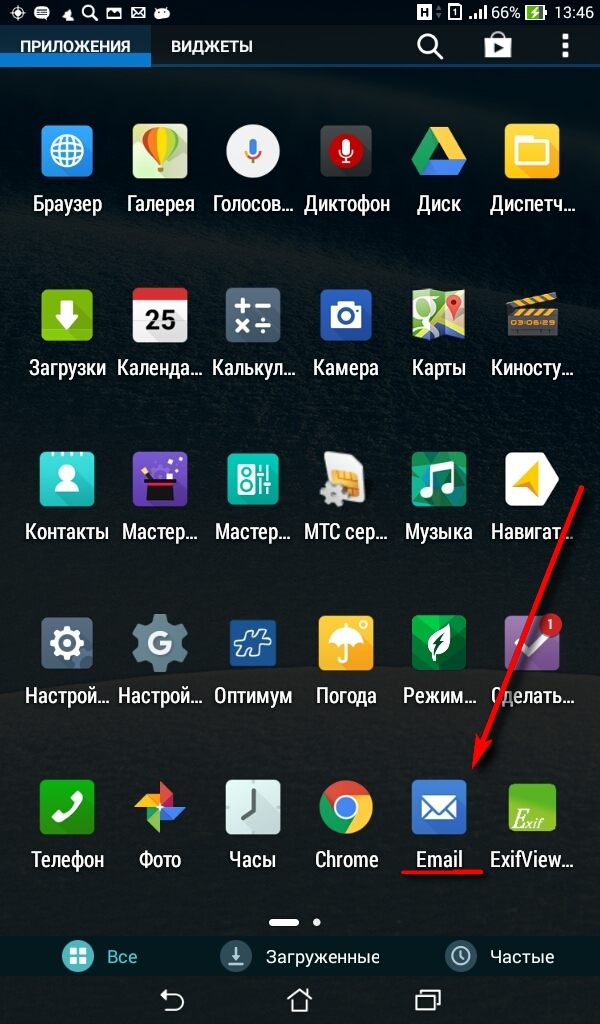
\includegraphics[width=0.3\linewidth]{pic_16.jpg} 
		\caption{Меню}\label{pic:pic_16}
	\end{figure}
	\item  Необходимо зайти в меню планшета найти и запустить приложение "Email" (рис.\ref{pic:pic_16}), в зависимости от версии Android и модели планшета иконка приложения может отличатся от представленной на рисунке. 
	\newpage 
	
	\begin{figure}[!h]
		\begin{floatrow}
			\ffigbox{\caption{Выбор провайдера эл.почты}\label{pic:pic_17}}%
			{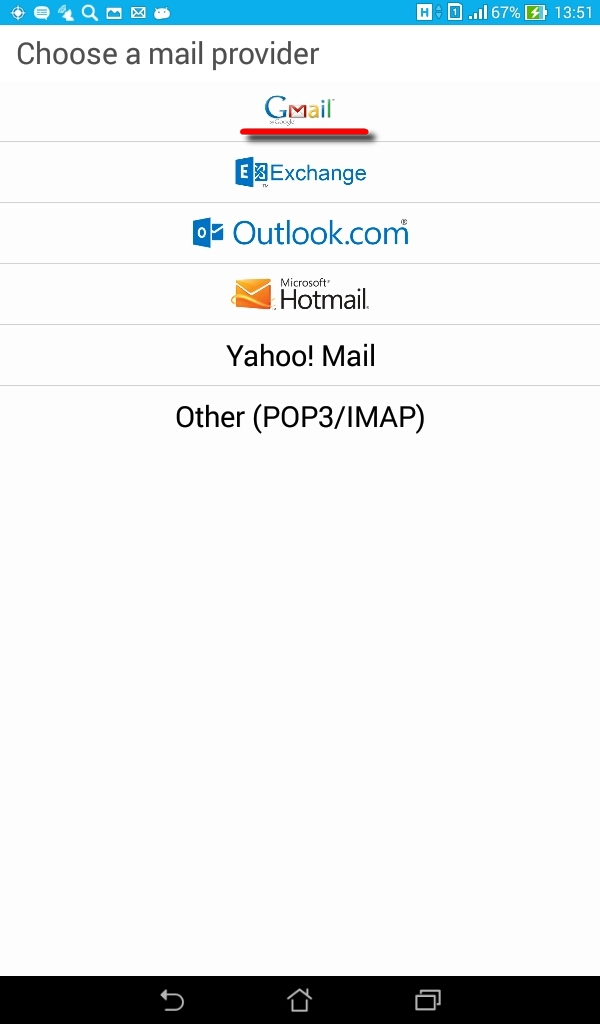
\includegraphics[width=0.58\linewidth]{pic_17.jpg}}
			\ffigbox{\caption{Выбор нужного аккаунта}\label{pic:pic_18}}%
			{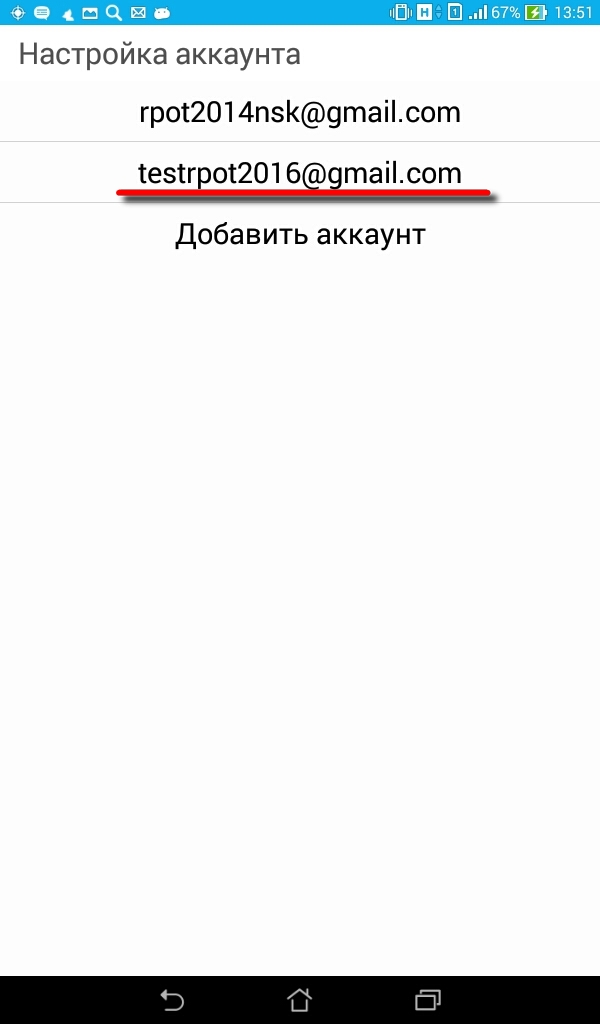
\includegraphics[width=0.58\linewidth]{pic_18.jpg}}         
		\end{floatrow}
	\end{figure}
	
	\item Выбрать нужного провайдера эл.почты, в нашем случае это "Gmail" (рис.\ref{pic:pic_17}):
	\item Из предложенного списка выбрать нужный аккаунт (рис.\ref{pic:pic_18}):

	
	\begin{figure}[!h]
		\begin{floatrow}
			\ffigbox{\caption{Ожидание входа}\label{pic:pic_19}}%
			{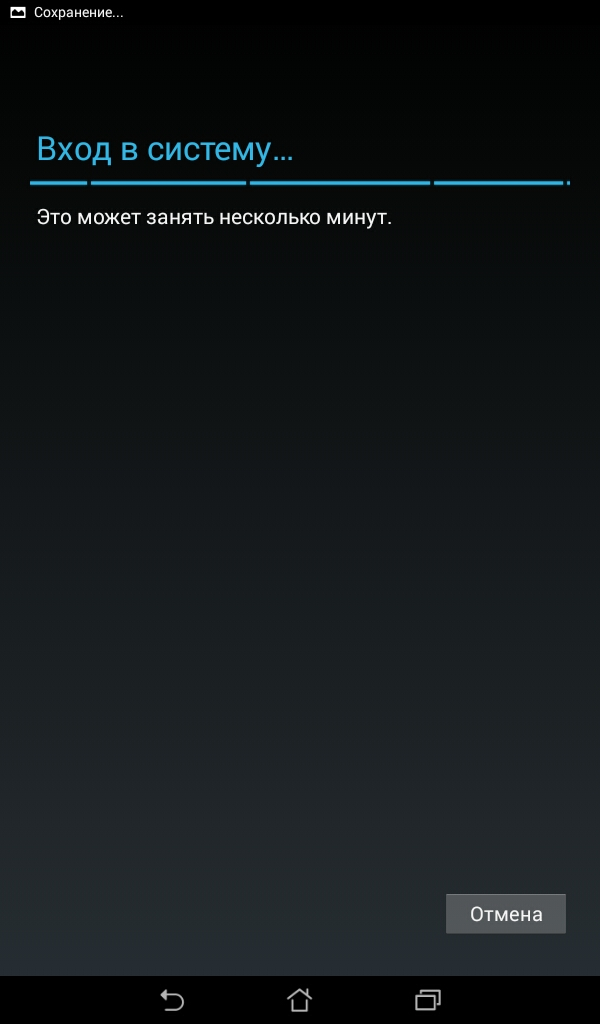
\includegraphics[width=0.58\linewidth]{pic_19.jpg}}
			\ffigbox{\caption{Подтверждение разрешений}\label{pic:pic_20}}%
			{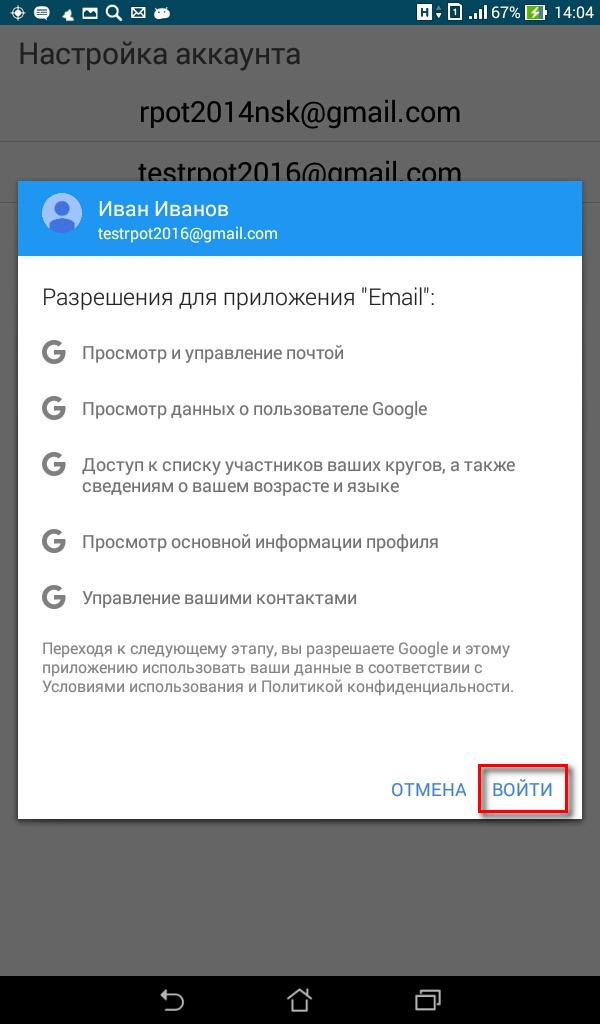
\includegraphics[width=0.58\linewidth]{pic_20.jpg}}         
		\end{floatrow}
	\end{figure}
	
	\item Далее некоторое время ожидаем входа в систему (рис.\ref{pic:pic_19}), после чего на запрос о разрешениях отвечаем "Войти" (рис.\ref{pic:pic_20}).


	\newpage 
	
	\begin{figure}[!h]
		\begin{floatrow}
			\ffigbox{\caption{Проверка настроек сервера}\label{pic:pic_21}}%
			{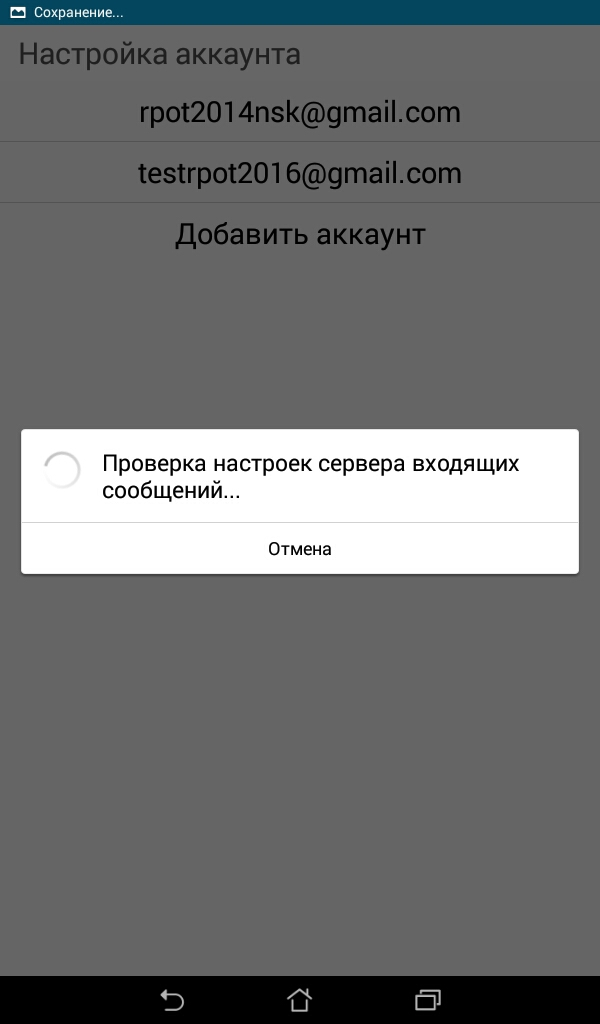
\includegraphics[width=0.58\linewidth]{pic_21.jpg}}
			\ffigbox{\caption{Настройки параметров аккаунта}\label{pic:pic_22}}%
			{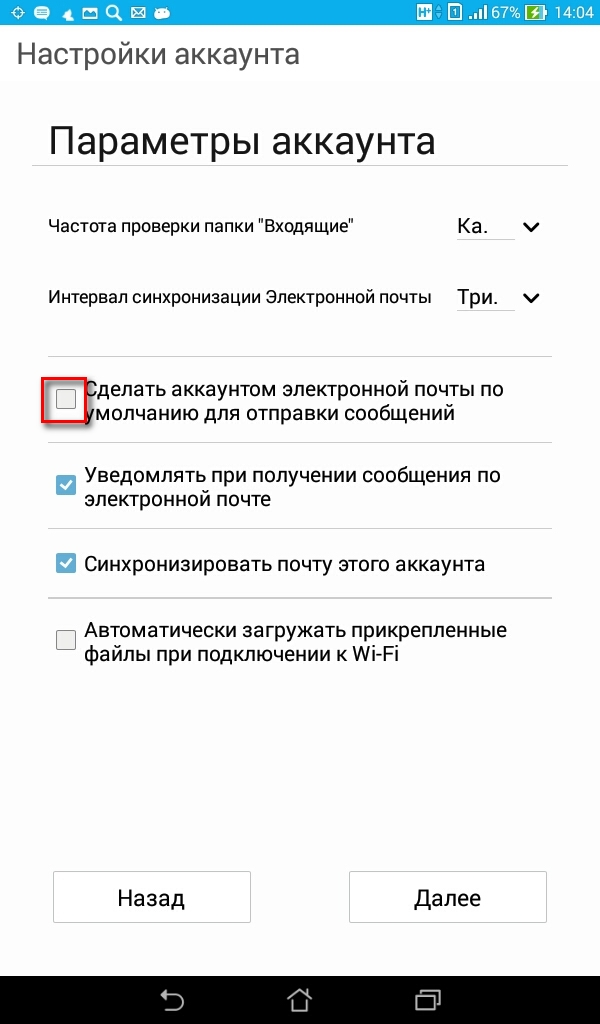
\includegraphics[width=0.58\linewidth]{pic_22.jpg}}         
		\end{floatrow}
	\end{figure}
	
	\item Дожидаемся пока Google проверит корректность настроек сервера (рис.\ref{pic:pic_21}) и затем проставив в настройка аккаунта галку "Сделать аккаунтом электронной почты по умолчанию"  (рис.\ref{pic:pic_22}), нажимаем "Далее"
	
	
	\begin{figure}[!h]
		\begin{floatrow}
			\ffigbox{\caption{Настроенный аккаунт}\label{pic:pic_23}}%
			{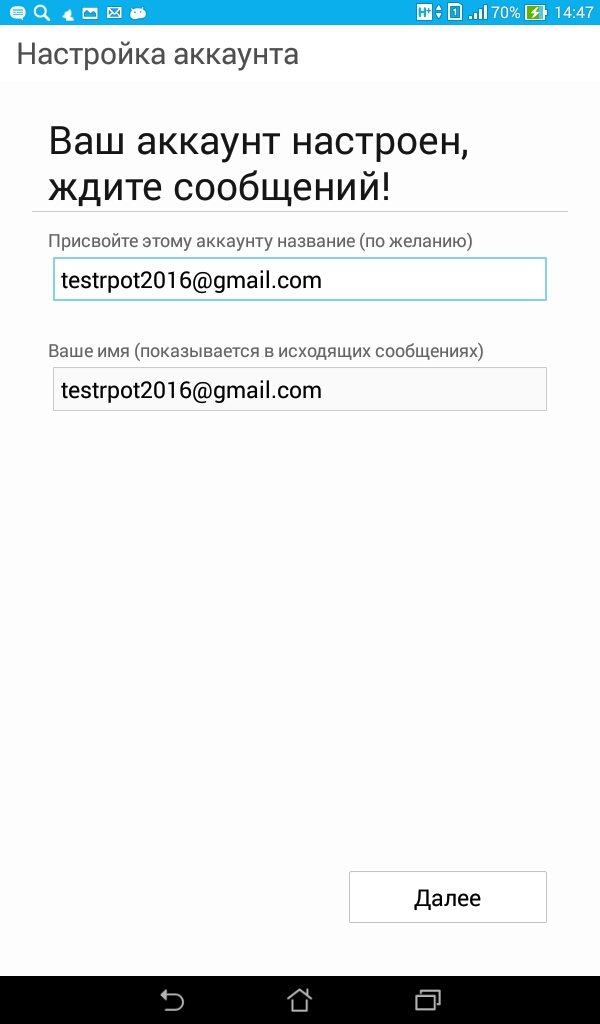
\includegraphics[width=0.58\linewidth]{pic_23.jpg}}
			\ffigbox{\caption{Синхронизация почты}\label{pic:pic_24}}%
			{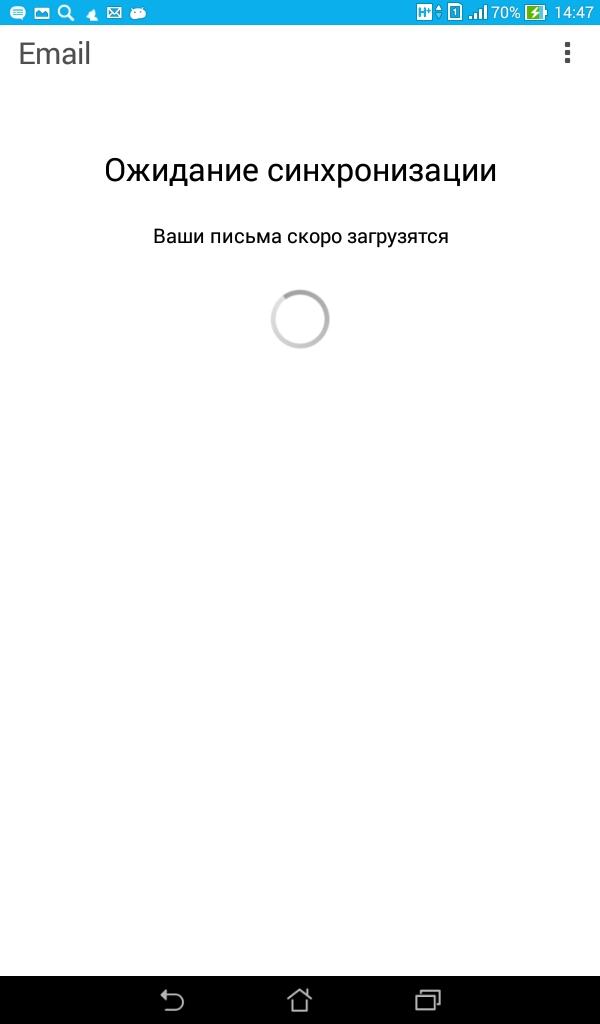
\includegraphics[width=0.58\linewidth]{pic_24.jpg}}         
		\end{floatrow}
	\end{figure}
	
	\item Читаем сообщение о том, что на аккаунт настроен, при желании корректируем доступные данные (рис.\ref{pic:pic_23}), дожидаемся проверки почты... (рис.\ref{pic:pic_24}).


\newpage
\begin{figure}[H]
	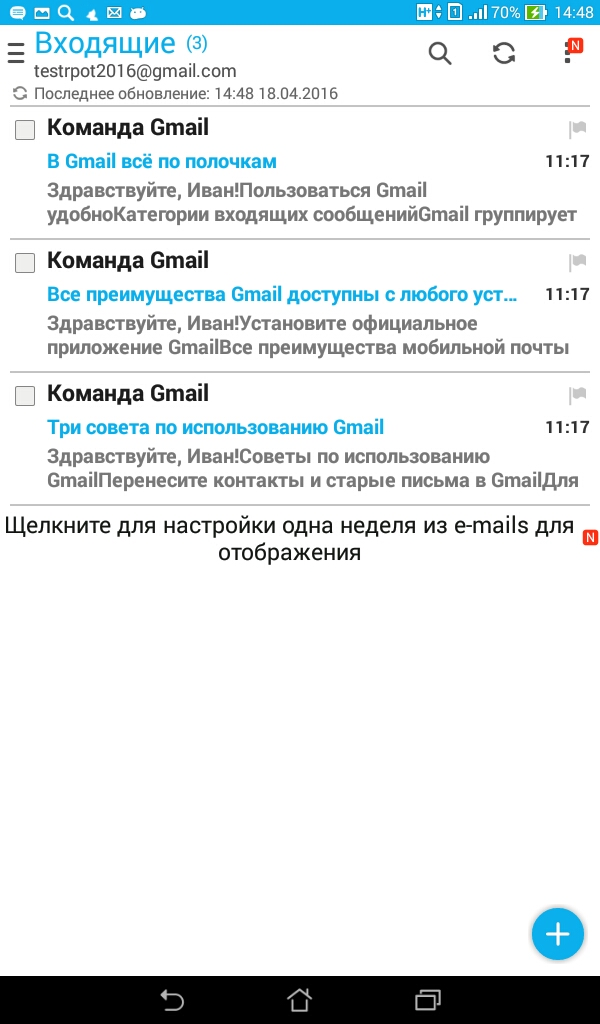
\includegraphics[width=0.3\linewidth]{pic_25.jpg} 
	\caption{Почтовый ящик}\label{pic:pic_25}
\end{figure}
\item Ваша программа электронной почты настроена. (рис.\ref{pic:pic_25}):


\end{enumerate}